\begin{problem}[1]
  Consider a 2-sphere with coordinates $(\theta, \phi)$ and a metric
  \[%
    \ds^2 = \dd{\theta}^2 + \sin^2(\theta) \dd{\phi}^2
  .\]%
  \begin{enumerate}
    \item Show that lines of constant longitude ($\phi =$ constant) are geodesics, and that the only line of constant latitude ($\theta =$ constant) that is a geodesic is the equator ($\theta = \pi/2$).
    \item Take a vector with components $V_\mu = (1, 0)$ and parallel-transport it once around a circle of constant latitude. What are the components of the resulting vector, as a function of $\theta$?
    \item Consider the following metric for one space-like and one time-like dimension:
      \[%
        \ds^2 = t^{-2}\left(-\dt^2 + \dx^2\right)
      .\]%
      Find all the Christoffel symbols, and then calculate the geodesics of this spacetime. \textit{Hint: for this second part, it is easiest to start with the definition of a geodesic as a maximum of proper time and find a relation for $x$ and $t$ by calculus of variance.}
  \end{enumerate}
\end{problem}

\begin{solution}[(i)]
  The geodesic equations are given by:
  \begin{equation}\label{eq:geodesic_equation}
    \ddot{x}^\mu + \Gamma_{\alpha\beta}^\mu \dot{x}^\alpha \dot{x}^\beta = 0
  \end{equation}
  For the given metric, we can compute the non-zero Christoffel symbols:
  \begin{align*}
    \Gamma_{\phi\phi}^\theta &= -\sin(\theta)\cos(\theta) \\
    \Gamma_{\theta\phi}^\phi &= \cot(\theta) = \Gamma_{\phi\theta}^\phi
  .\end{align*}
  Now, let's consider lines of constant longitude, i.e., $\phi = \text{constant}$. In this case, $\dot{\phi} = 0$, and the geodesic equations reduce to:
  \begin{align*}
    \ddot{\theta} + \Gamma_{\theta\theta}^\theta \dot{\theta}^2 &= 0 \\
    \ddot{\phi} + \Gamma_{\theta\phi}^\phi \dot{\theta}\dot{\phi} &= 0
  .\end{align*}
  Since $\dot{\phi} = 0$, the second equation is automatically satisfied. The first equation simplifies to $\ddot{\theta} = 0$, which means that $\theta$ changes linearly with the affine parameter, confirming that lines of constant longitude are geodesics.

  Next, let's consider lines of constant latitude, i.e., $\theta = \text{constant}$. In this case, $\dot{\theta} = 0$, and the geodesic equations reduce to:
  \begin{align*}
    \ddot{\theta} + \Gamma_{\phi\phi}^\theta \dot{\phi}^2 &= 0 \\
    \ddot{\phi} + \Gamma_{\theta\phi}^\phi \dot{\theta}\dot{\phi} &= 0
  .\end{align*}
  Since $\dot{\theta} = 0$, the second equation is automatically satisfied. The first equation simplifies to:
  \[%
    \Gamma_{\phi\phi}^\theta \dot{\phi}^2 = 0
  .\]%
  This implies that either $\dot{\phi} = 0$ (which is trivial) or $\Gamma_{\phi\phi}^\theta = 0$. The latter condition holds only when $\theta = \pi/2$, which corresponds to the equator. Therefore, the only line of constant latitude that is a geodesic is the equator.
\end{solution}

\begin{solution}[(ii)]
  Instead of working with covariant components, it's easier to work with contravariant components for parallel transport. For the inverse metric, we have:
  \[%
    g^{\theta\theta} = 1 \aand g^{\phi\phi} = \frac{1}{\sin^2(\theta)}
  .\]%
  Raising the indices using the inverse metric components, we have:
  \[%
    V^\theta = g^{\theta\theta} V_\theta = 1 \cdot 1 = 1 \aand V^\phi = g^{\phi\phi} V_\phi = \frac{1}{\sin^2(\theta)} \cdot 0 = 0
  .\]%
  Thus, we have the initial contravariant components $V^\mu = (1, 0)$. Using the equations for parallel transport of contravariant components:
  \begin{equation}\label{eq:parallel_transport}
    \odv{V^\mu}{\lambda} + \Gamma_{\alpha\beta}^\mu V^\alpha \odv{x^\beta}{\lambda} = 0
  \end{equation}
  Parametrizing the curve as $x^\mu = (\theta, \phi(\lambda))$ with $\theta$ constant, we have $\dot{x}^\mu = (0, \dot{\phi})$. Thus, the equations for parallel transport become:
  \begin{gather*}
    \odv{V^\theta}{\lambda} + \Gamma_{\phi\phi}^\theta V^\phi \dot{\phi} = 0 \\
    \odv{V^\phi}{\lambda} + \Gamma_{\theta\phi}^\phi V^\theta \dot{\phi} = 0
  .\end{gather*}
  Substituting the non-zero Christoffel symbols from part (i), we get:
  \begin{gather*}
    \odv{V^\theta}{\lambda} - \sin(\theta)\cos(\theta) V^\phi \dot{\phi} = 0 \\
    \odv{V^\phi}{\lambda} + \cot(\theta) V^\theta \dot{\phi} = 0
  .\end{gather*}
  Letting $\dot{\phi} = \omega$ (a constant), we can rewrite the equations as:
  \begin{gather}
    \odv{V^\theta}{\lambda} - \sin(\theta)\cos(\theta) V^\phi \omega = 0\label{eq:1} \\
    \odv{V^\phi}{\lambda} + \cot(\theta) V^\theta \omega = 0\label{eq:2}
  .\end{gather}
  Solving for $V^\theta$ from Equation~\eqref{eq:1}, we get:
  \[%
    V^\theta(\lambda) = \sin(\theta)\cos(\theta) \omega \int V^\phi(\lambda) \dd{\lambda}
  ,\]%
  where we're treating $\sin(\theta)$, $\cos(\theta)$, and $\omega$ as constants. Substituting this expression for $V^\theta$ into Equation~\eqref{eq:2}, we have:
  \begin{equation}\label{eq:3}
    \odv{V^\phi}{\lambda} + \cot(\theta) \left(\sin(\theta)\cos(\theta) \omega \int V^\phi(\lambda) \dd{\lambda}\right) \omega = 0
  \end{equation}
  Differentiating Equation~\eqref{eq:3} with respect to $\lambda$, we obtain a second-order differential equation for $V^\phi$:
  \[%
    \odv[2]{V^\phi}{\lambda} + \omega^2\cos^2(\theta) V^\phi = 0
  .\]%
  This is a simple harmonic oscillator equation with general solution:
  \[%
    V^\phi(\lambda) = A \cos(\omega \cos(\theta) \lambda) + B \sin(\omega \cos(\theta) \lambda)
  .\]%
  We now solve for $A$ and $B$ given the initial conditions. At $\lambda = 0$, we have $V^\phi(0) = 0$, which implies $A = 0$. To find $B$, we differentiate $V^\phi$:
  \[%
    \odv{V^\phi}{\lambda} = B \omega \cos(\theta) \cos(\omega \cos(\theta) \lambda)
  .\]%
  By Equation~\eqref{eq:parallel_transport}, at $\lambda = 0$, we have:
  \[%
    \odv{V^\phi}{\lambda}\bigg|_{\lambda=0} + \cot(\theta) V^\theta(0) \omega = 0
  .\]%
  Since $V^\theta(0) = 1$, we have:
  \[%
    B \omega \cos(\theta) + \cot(\theta) \omega = 0 \implies B = -\frac{\cot(\theta)}{\cos(\theta)} = -\csc(\theta)
  .\]%
  Thus, the solution for $V^\phi$ is:
  \[%
    V^\phi(\lambda) = -\csc(\theta) \sin(\omega \cos(\theta) \lambda)
  .\]%
  Plugging this back into Equation~\eqref{eq:1}, we can solve for $V^\theta$:
  \begin{align*}
    V^\theta(\lambda) &= \sin(\theta)\cos(\theta) \omega \int -\csc(\theta) \sin(\omega \cos(\theta) \lambda) \dd{\lambda} \\
                      &= -\omega\cos(\theta) \left(-\frac{\sec(\theta)\cos(\omega \cos(\theta) \lambda)}{\omega}\right) \\
                      &= \cos(\omega \cos(\theta) \lambda)
  .\end{align*}
  Therefore, the components of the resulting vector after parallel transport around a circle of constant latitude are:
  \[%
    V^\mu(\lambda) = \left(\cos(\omega \cos(\theta) \lambda), -\csc(\theta) \sin(\omega \cos(\theta) \lambda)\right)
  .\]%
  To express the result in terms of the angle $\phi$, we note that $\phi = \omega \lambda$. Thus, the final components are:
  \[%
    V^\mu(\phi) = \left(\cos(\phi \cos(\theta)), -\csc(\theta) \sin(\phi \cos(\theta))\right)
  .\qedhere\]%
\end{solution}

\begin{solution}[(iii)]
  Given the metric, we have:
  \[%
    g_{tt} = -t^{-2}, \quad g_{xx} = t^{-2}
  .\]%
  The non-zero Christoffel symbols can be computed as follows:
  \begin{align*}
    \Gamma_{tt}^t &= \frac{1}{2} g^{t\mu}(\partial_t g_{\mu t} + \partial_t g_{t\mu} - \partial_\mu g_{tt}) = \frac{1}{2} g^{tt}(-2t^{-3}) = -\frac{1}{t} \\
    \Gamma_{tx}^t &= \frac{1}{2} g^{tt}(\partial_x g_{t t} + \partial_t g_{xt} - \partial_t g_{tx}) = 0 \\
    \Gamma_{xx}^t &= \frac{1}{2} g^{tt}(\partial_x g_{tx} + \partial_x g_{xt} - \partial_t g_{xx}) = -\frac{1}{2} g^{tt}(2t^{-3}) = -\frac{1}{t} \\
    \Gamma_{tt}^x &= \frac{1}{2} g^{xx}(\partial_t g_{xt} + \partial_t g_{tx} - \partial_x g_{tt}) = 0 \\
    \Gamma_{tx}^x &= \frac{1}{2} g^{xx}(\partial_x g_{xt} + \partial_t g_{xx} - \partial_x g_{tx}) = \frac{1}{2} g^{xx}(-2t^{-3}) = -\frac{1}{t} \\
    \Gamma_{xx}^x &= \frac{1}{2} g^{xx}(\partial_x g_{xx} + \partial_x g_{xx} - \partial_x g_{xx}) = 0
  .\end{align*}
  Thus, the non-zero Christoffel symbols are:
  \[%
    \Gamma_{tt}^t = -\frac{1}{t}, \quad \Gamma_{xx}^t = -\frac{1}{t}, \quad \Gamma_{tx}^x = -\frac{1}{t} = \Gamma_{xt}^x
  .\]%
  Using Equation~\eqref{eq:geodesic_equation}, we can write the geodesic equations for $t$ and $x$:
  \begin{align*}
    \mu = t:\quad& \ddot{t} + \Gamma_{tt}^t \dot{t}^2 + 2\Gamma_{xx}^t \dot{t}\dot{x} + \Gamma_{xx}^t \dot{x}^2 = 0 \\
                 & \ddot{t} - \frac{1}{t} \dot{t}^2 - \frac{1}{t} \dot{x}^2 = 0 \\
    \mu = x:\quad& \ddot{x} + \Gamma_{tx}^x \dot{x}\dot{t} + \Gamma_{xt}^x \dot{t}\dot{x} = 0 \\
                 & \ddot{x} - \frac{2}{t} \dot{t}\dot{x} = 0
  .\end{align*}
  Therefore, the geodesic equations for this spacetime are:
  \begin{gather*}
    \ddot{t} - \frac{1}{t} \dot{t}^2 - \frac{1}{t} \dot{x}^2 = 0 \\
    \ddot{x} - \frac{2}{t} \dot{t}\dot{x} = 0
  .\qedhere\end{gather*}
\end{solution}

\begin{problem}[2]
  Consider the following line element,
  \[%
    \ds^2 = -\left(1 - \frac{2M}{\sqrt{r^2 + b^2}}\right)\dt^2 + \left(1 - \frac{2M}{\sqrt{r^2 + b^2}}\right)^{-1} \dr^2 + \left(r^2 + b^2\right)\left(\dd{\theta}^2 + \sin^2(\theta)\dd{\phi}^2\right)
  ,\]%
  where $M$ and $b$ are positive, real constants. Note that we are using geometrical units where $G = c = 1$.
  \begin{enumerate}
    \item Write down the metric and the inverse metric in the $(t, r, \theta, \phi)$ coordinate system.
    \item Write down the non-zero Christoffel symbols $\Gamma_{\beta\gamma}^\alpha$ for this metric. \textit{Hint: although there are 40 Christoffel symbols that are distinct by taking account of the symmetry under $\beta \leftrightarrow \gamma$, only 9 are non-zero.}
    \item Write the geodesic equation in this metric for a massive particle, i.e. write equations for $\ddot{t}$, $\ddot{r}$, $\ddot{\theta}$, $\ddot{\phi}$ where the double-dots are with respect to proper time $\tau$.
    \item Calculate the effective potential for timelike orbits for arbitrary $M$ and $b$.
    \item Do bound orbital solutions exist for $M = 0$? Why or why not?
    \item ($\star$) Build a numerical solver for integrating the geodesic equation given an initial position $\epsilon$ and $\ell$. Here, $\epsilon$ corresponds to energy density as written in class. Can you find any interesting geometries and/or trajectories?
  \end{enumerate}
\end{problem}

\begin{solution}[(i)]
  The metric components in the $(t, r, \theta, \phi)$ coordinate system are given by:
  \[%
    g_{tt} = -\left(1 - \frac{2M}{\sqrt{r^2 + b^2}}\right), \quad g_{rr} = \left(1 - \frac{2M}{\sqrt{r^2 + b^2}}\right)^{-1}, \quad g_{\theta\theta} = r^2 + b^2, \quad g_{\phi\phi} = (r^2 + b^2)\sin^2(\theta)
  .\]%
  All off-diagonal components are zero. Thus, the metric tensor can be written as:
  \[%
    g_{\mu\nu} = \begin{pmatrix}
      -\left(1 - \frac{2M}{\sqrt{r^2 + b^2}}\right) & 0 & 0 & 0 \\
      0 & \left(1 - \frac{2M}{\sqrt{r^2 + b^2}}\right)^{-1} & 0 & 0 \\
      0 & 0 & r^2 + b^2 & 0 \\
      0 & 0 & 0 & (r^2 + b^2)\sin^2(\theta)
    \end{pmatrix}
  .\]%
  The inverse metric components can be computed as follows:
  \[%
    g^{tt} = -\left(1 - \frac{2M}{\sqrt{r^2 + b^2}}\right)^{-1}, \quad g^{rr} = \left(1 - \frac{2M}{\sqrt{r^2 + b^2}}\right), \quad g^{\theta\theta} = \frac{1}{r^2 + b^2}, \quad g^{\phi\phi} = \frac{1}{(r^2 + b^2)\sin^2(\theta)}
  .\]%
  Thus, the inverse metric tensor can be written as:
  \[%
    g^{\mu\nu} = \begin{pmatrix}
      -\left(1 - \frac{2M}{\sqrt{r^2 + b^2}}\right)^{-1} & 0 & 0 & 0 \\
      0 & \left(1 - \frac{2M}{\sqrt{r^2 + b^2}}\right) & 0 & 0 \\
      0 & 0 & \frac{1}{r^2 + b^2} & 0 \\
      0 & 0 & 0 & \frac{1}{(r^2 + b^2)\sin^2(\theta)}
    \end{pmatrix}
  .\qedhere\]%
\end{solution}

\begin{solution}[(ii)]
  After computing all the Christoffel symbols using the metric components from part (i), we find that the non-zero Christoffel symbols are:
  \begin{gather*}
    \Gamma_{rt}^t = \frac{1}{2}g^{tt}\pd{r}g_{tt} = \Gamma_{tr}^t \\
    \Gamma_{tt}^r = -\frac{1}{2}g^{rr}\pd{r}g_{tt}, \quad \Gamma_{rr}^r = -\frac{1}{2}g^{rr}\pd{r}g_{rr}, \quad \Gamma_{\theta\theta}^r = -\frac{1}{2}g^{rr}\pd{r}g_{\theta\theta}, \quad \Gamma_{\phi\phi}^r = -\frac{1}{2}g^{rr}\pd{r}g_{\phi\phi} \\
    \Gamma_{r\theta}^\theta = \frac{1}{2}g^{\theta\theta}\pd{r}g_{\theta\theta} = \Gamma_{\theta r}^\theta, \quad \Gamma_{\phi\phi}^\theta = -\frac{1}{2}g^{\theta\theta}\pd{\theta}g_{\phi\phi} \\
    \Gamma_{r\phi}^\phi = \frac{1}{2}g^{\phi\phi}\pd{r}g_{\phi\phi} = \Gamma_{\phi r}^\phi, \quad \Gamma_{\theta\phi}^\phi = \frac{1}{2}g^{\phi\phi}\pd{\theta}g_{\phi\phi} = \Gamma_{\phi\theta}^\phi
  .\qedhere\end{gather*}
\end{solution}

\begin{solution}[(iii)]
  The only geodesic equation for the $t$ coordinate is:
  \[%
    \ddot{t} + g^{tt}\pd{r}g_{tt} \dot{t}\dot{r} = 0
  .\]%
  The geodesic equation for the $r$ coordinate is:
  \[%
    \ddot{r} - \frac{1}{2}g^{rr}\pd{r}g_{tt} \dot{t}^2 - \frac{1}{2}g^{rr}\pd{r}g_{rr} \dot{r}^2 - rg^{rr} \dot{\theta}^2 - rg^{rr}\sin^2(\theta) \dot{\phi}^2 = 0
  .\]%
  The geodesic equation for the $\theta$ coordinate is:
  \[%
    \ddot{\theta} + \frac{2}{r} \dot{r}\dot{\theta} - \sin(\theta)\cos(\theta) \dot{\phi}^2 = 0
  .\]%
  The geodesic equation for the $\phi$ coordinate is:
  \[%
    \ddot{\phi} + \frac{2}{r} \dot{r}\dot{\phi} + 2\cot(\theta) \dot{\theta}\dot{\phi} = 0
  .\]%
  Thus, the geodesic equations for a massive particle in this metric are:
  \begin{gather*}
    \ddot{t} + g^{tt}\pd{r}g_{tt} \dot{t}\dot{r} = 0 \\
    \ddot{r} - \frac{1}{2}g^{rr}\pd{r}g_{tt} \dot{t}^2 - \frac{1}{2}g^{rr}\pd{r}g_{rr} \dot{r}^2 - rg^{rr} \dot{\theta}^2 - rg^{rr}\sin^2(\theta) \dot{\phi}^2 = 0 \\
    \ddot{\theta} + \frac{2}{r} \dot{r}\dot{\theta} - \sin(\theta)\cos(\theta) \dot{\phi}^2 = 0 \\
    \ddot{\phi} + \frac{2}{r} \dot{r}\dot{\phi} + 2\cot(\theta) \dot{\theta}\dot{\phi} = 0
  .\qedhere\end{gather*}
\end{solution}

\begin{solution}[(iv)]
  For a massive particle in a static, spherically symmetric metric,
  \[%
    \ds^2 = -f(r)\dt^2 + h(r)\dr^2 + r^2 \left(\dd{\theta}^2 + \sin^2(\theta)\dd{\phi}^2\right)
  ,\]%
  the conserved quantities are:
  \[%
    E = f(r)\dot{t}, \qquad L = r^2 \dot{\phi}
  ,\]%
  and we consider motion in the equatorial plane $\theta = \pi/2$. The timelike condition $g_{\mu\nu}\dot{x}^\mu \dot{x}^\nu = -1$ gives:
  \[%
    -1 = -f(r)\dot{t}^2 + h(r) \dot{r}^2 + r^2 \dot{\phi}^2
  .\]%
  Substituting the conserved quantities, we find:
  \[%
    \dot{r}^2 = \frac{E^2}{f(r)h(r)} - \frac{1}{h(r)}\left(1 + \frac{L^2}{r^2}\right)
  .\]%
  Define $V_{\text{eff}}(r)$ such that:
  \[%
    \frac{1}{2}\dot{r}^2 + V_{\text{eff}}(r) = \frac{E^2}{2}
  ,\]%
  giving us:
  \[%
    V_{\text{eff}}(r) = \frac{1}{2} \left(1 + \frac{L^2}{r^2}\right) \frac{1}{h(r)}
  .\]%
  In the case where $h(r) = 1/f(r)$, e.g. for the metric:
  \[%
    f(r) = 1 - \frac{2M}{r} + \frac{b}{r^2}
  ,\]%
  the effective potential becomes:
  \[%
    V_{\text{eff}}(r) = f(r) \left(1 + \frac{L^2}{r^2}\right) = \left(1 - \frac{2M}{r} + \frac{b}{r^2}\right) \left(1 + \frac{L^2}{r^2}\right)
  .\]%
  This potential determines the radial motion of a timelike particle with energy $E$ and angular momentum $L$.
\end{solution}

\begin{solution}[(v)]
  To determine whether bound orbits exist for $M = 0$, we examine the effective potential for timelike particles:
  \[%
    V_{\text{eff}}(r) = \left(1 - \frac{2M}{r} + \frac{b}{r^2}\right) \left(1 + \frac{L^2}{r^2}\right)
  .\]%
  Setting $M = 0$, the potential reduces to:
  \begin{equation}\label{eq:effective_potential_M0}
    V_{\text{eff}}(r) = \left(1 + \frac{b}{r^2}\right) \left(1 + \frac{L^2}{r^2}\right) = 1 + \frac{L^2 + b}{r^2} + \frac{bL^2}{r^4}
  \end{equation}
  For a bound orbit to exist, the effective potential must have a local minimum at some finite $r > 0$, so that the radial motion oscillates between two turning points. We check for extrema by differentiating Equation~\eqref{eq:effective_potential_M0} with respect to $r$:
  \begin{equation}\label{eq:derivative_effective_potential}
    \odv{V_{\text{eff}}}{r} = -2\frac{L^2 + b}{r^3} - 4 \frac{bL^2}{r^5} = -\frac{2(L^2 + b) r^2 + 4 bL^2}{r^5}
  \end{equation}
  Setting Equation~\eqref{eq:derivative_effective_potential} to zero to find critical points, we have:
  \[%
    2(L^2 + b) r^2 + 4 bL^2 = 0 \implies r^2 = -\frac{2bL^2}{L^2 + b}
  .\]%
  Since $r^2 > 0$, this equation has no real solutions for any real $L$ and $b$, except possibly for negative $b$ with $|b| < L^2$, which depends on the spacetime. In the usual case of positive $b$ (repulsive term), there is no local minimum. Therefore, when $M = 0$, the effective potential is monotonically decreasing or always repulsive, and there is no finite radius at which a particle can be trapped.
\end{solution}

\begin{solution}[(vi)]
  To study the motion of timelike geodesics in the given spacetime, we numerically integrated the geodesic equations derived in part (iii).  We worked in the equatorial plane $\theta = \pi/2$ without loss of generality, which reduces the system to the three variables $(t(\tau), r(\tau), \phi(\tau))$ with initial energy density $\epsilon$ and angular momentum per unit mass $\ell$.

  The system of ODEs was evolved using a standard fourth–order Runge--Kutta integrator. From the numerical solution, we reconstructed the Cartesian coordinates
  \[%
    x(\tau) = r(\tau)\cos\phi(\tau), \quad y(\tau) = r(\tau)\sin\phi(\tau)
  ,\]%
  which give a spatial visualization of the orbit. A representative trajectory is shown below:
  \begin{center}
    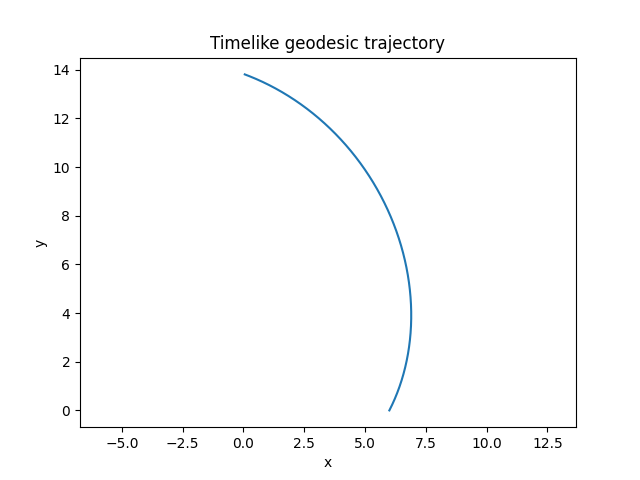
\includegraphics[width=0.6\textwidth]{image-files/timelike-geodesic.png}
  \end{center}

  The resulting orbit displays a smooth inward-curving trajectory, typical of spacetimes with an effective attractive potential. The numerical integrator confirms the behavior predicted by the effective potential. For generic nonzero $M$ a range of interesting timelike trajectories exists, while the $M = 0$ limit becomes purely repulsive in the radial direction and no bound orbits are observed, consistent with the analysis in part (v).
\end{solution}
